\section{Mixed Practice}
\subsection{Warm Ups}
These are good problems for reinforcing the vocabulary and foundational concepts of this chapter. 

\begin{exercise}{Reference Sheet \Coffeecup}
Make sure your power series reference sheet is completely filled out.  Once you do, see if you can rewrite it correctly from memory without looking at the original.  It is essential to have those formulas internalized in order to be proficient with power series.
\end{exercise}

\subsection{Sample Test Problems}

\begin{exercise}{\Coffeecup \Coffeecup }
By hand, (or using your custom built Arduino calculator) compute the cubed root of $e$ accurate to one place past the decimal. (That is, error less that one one-tenth)  Use Taylor's error theorem to justify your answer is correct!
\AnswerKeyEntry{$1.4$}
\solushun{Note: $\sqrt[3]{e}= e^{1/3}$ Thus we need to substitute $x= \frac{1}{3} $ into $f(x) = e^{x}= \sum\limits_{n=0}^{\infty}{\frac{x^n}{n!}}$ This means $a=0$.  Also we have $f^{n+1} =e^x$ which has its max at $\frac{1}{3}$ on the interval $[0,\frac{1}{3}]$.  We don't know the value of $e^{1/3}$ since its what we are trying to compute but we can infer the value from the fact that $e<2^3=8$ which means that $e^{1/3} <2$  Therefore we can use $M=2$ as a safe estimator in our error formula.  Thus the error in a degree $n$ approximation will be $\frac{M \cdot |x-a|^{n+1}}{(n+1)!}=\frac{2 \left|\frac{1}{3}-0\right|^{n+1}}{(n+1)!}=\frac{2}{3^{n+1}(n+1)!}$ which we need to be less and 0.1. We can look at this in a table:
\begin{center}
\begin{tabular}{|c|c|} \hline
$n$ & $\frac{2}{3^{n+1}(n+1)!}$  \\ \hline
 1 & $\frac{2}{3^{2}(2)!}=\frac{1}{9} $  \\ 
 2 &  $\frac{2}{3^{3}(3)!} = \frac{1}{81}<\frac{1}{10}$ \\
 3 &  $\frac{2}{3^{4}(4)!} = \frac{1}{972}<\frac{1}{100}$ \\
\end{tabular}
\end{center}
So we use $n=2$ to compute:$e^{1/3} = 1+ \frac{1}{3} + \frac{\left(\frac{1}{3}\right)^2}{2!}= 1+ \frac{1}{3} +\frac{1}{18} = 1+ 0.3333 \dotfill  + 0.05555 \dotfill \approx 1.4$\\}{0in}
\end{exercise}

\begin{exercise}{\Coffeecup \Coffeecup }
 For each of the following, identify whether the sum converges to a real number or if it diverges.  If it converges, find a closed form for the real number it converges to.  You may cite results stated in class or in homework.
\begin{enumerate}[label=\alph*.)]
\item $1+\binom{1/2}{1}+\frac{\left(\binom{1/2}{1}\right)^2}{2!}+\frac{\left(\binom{1/2}{1}\right)^3}{3!}+\frac{\left(\binom{1/2}{1}\right)^4}{4!}+\cdots $
\solushun{$1+\binom{1/2}{1}+\frac{\left(\binom{1/2}{1}\right)^2}{2!}+\frac{\left(\binom{1/2}{1}\right)^3}{3!}+\frac{\left(\binom{1/2}{1}\right)^4}{4!}+\cdots  = 1 + \frac{\left(\frac{1}{2}\right)}{2!}+\frac{\left(\frac{1}{2}\right)^2}{3!}+\frac{\left(\frac{1}{2}\right)^3}{4!}+\cdot = \sum\limits_{n=0}^{\infty} \frac{\left(\frac{1}{2}\right)^{n}}{n!} = e^{1/2}=\sqrt{e}$
\\ }{0in}

\item $1+\binom{1/2}{1}+\binom{1/2}{2}+\binom{1/2}{3}+\binom{1/2}{4}+\cdots $
\solushun{$1+\binom{1/2}{1}+\binom{1/2}{2}+\binom{1/2}{3}+\binom{1/2}{4}+\cdots=
\sum\limits_{n=0}^{\infty}{\binom{1/2}{n} 1^{n}}=(1+1)^{1/2} = \sqrt{2}$
\\ }{0in}

\item $0.20202020202020\ldots$ 
\solushun{$0.20202020202020\ldots= \frac{20}{100} + \frac{20}{10000} + \frac{20}{1000000}+ \cdot = 0.2\left(1+ \frac{1}{100} + \frac{1}{10000} + \frac{1}{1000000}+ \cdot\right) = 0.2\sum_{n=0}^{\infty}{\left(\frac{1}{100}\right)^{n}}$ This is a Geometric Series so $0.2\sum_{n=0}^{\infty}{\left(\frac{1}{100}\right)^{n}}=\frac{2}{10}\cdot \frac{1}{1-\frac{1}{100}}= \frac{2}{10}\frac{100}{99} = \frac{20}{99}$ 
\\ }{0in}

\item $5+5^2/1!+5^3/2!+5^4/3!+5^5/4!+\cdots $
\solushun{$5+5^2/1!+5^3/2!+5^4/3!+5^5/4!+\cdots =5\left(1+5/1!+5^2/2!+5^3/3!+5^4/4!+\cdots\right)= 5 \sum\limits_{n = 0}^{\infty}{\frac{5^n}{n!}} = 5e^5 $
\\ }{0in}
\end{enumerate}
\AnswerKeyEntry{a.) $\sqrt{e}$,~~b.) $\sqrt{2}$,~~c.) $\frac{20}{99}$,~~d.) $5e^5$}

\end{exercise}

\begin{exercise}{\Coffeecup \Coffeecup }
Consider the following limit: 
$$ \lim\limits_{x\rightarrow 0} \frac{x^2}{\sec(x)-1}$$

\begin{enumerate}[label=\alph*.)]
\item Evaluate the limit by L'Hospital's Rule.
\solushun{ $ \lim\limits_{x\rightarrow 0} \frac{x^2}{sec(x)-1} \stackrel{\text{H}}{=} \lim\limits_{x\rightarrow 0} \frac{2x}{\sec{x}\tan{x}} \stackrel{\text{H}}{=} =\lim\limits_{x\rightarrow 0} \frac{2}{\sec{x}\tan^{2}{x}+\sec^3{x}}\frac{2}{0+1} = 2$
\\ }{0in}

\item Evaluate the limit by replacing $\sec(x)$ with its power series centered at zero.  (HINT: You only need a few terms of this series in order to evaluate the limit!)  Verify that your results match.
\solushun{Brute force a degree 2 power series for $\sec{x}=a_0+a_1 x+a_2 x^2$.\\
Set $x=0$ then $\sec{0} = a_0 \longleftrightarrow a_0 = 1$\\
Differentiate: $\sec{x}\tan{x} = a_1+2a_2 x$ Set $x=0\longleftrightarrow 0 = a_1$\\
Differentiate: $\sec{x}\tan^2{x} + \sec^3{x} = 2a_2$ Set $x=0 \longleftrightarrow 0+1 = 2a_2 \longleftrightarrow a_2 = \frac{1}{2}$ thus\\
$\lim\limits_{x\rightarrow 0} \frac{x^2}{sec(x)-1} = \lim\limits_{x\rightarrow 0} \frac{x^2}{1+\frac{1}{2}x^2} = \lim\limits_{x\rightarrow 0} \frac{1}{\frac{1}{x^2}+\frac{1}{2}}= \frac{1}{\frac{1}{2}} = 2$
\\ }{0in}

\end{enumerate}
\AnswerKeyEntry{a.~~ 2 
b.~~ $\lim\limits_{x\rightarrow 0} \frac{x^2}{1+\frac{1}{2}x^2} =2$ 
}
\end{exercise}

\begin{exercise}{\Coffeecup \Coffeecup }
Consider the function $$ f(x) = \sqrt{1+x^2}$$
\begin{enumerate}[label=\alph*.)]
\item Explain why the graph of the function above is equivalent to just the top half of the hyperbola $y^2-x^2=1 $.
\solushun{Because $y^2-x^2=1 \rightarrow y^2=1+x^2 \rightarrow y =\pm\sqrt{1+x^2}$
\\ }{0in}

\item Show that $f(x)$ has slant asymptotes at $y=\pm x$ by computing the limits:

$$\lim_{x\rightarrow \infty} \frac{f(x)}{x} $$
and
$$\lim_{x\rightarrow -\infty} \frac{f(x)}{-x} $$
\solushun{$\lim\limits_{x\rightarrow \infty} \frac{f(x)}{x}=\lim\limits_{x\rightarrow \infty} \frac{\sqrt{1+x^2}}{x}=\lim\limits_{x\rightarrow \infty} \sqrt{\frac{1+x^2}{x^2}}=\lim\limits_{x\rightarrow \infty} \sqrt{\frac{1/x^2+1}{1}}=1$\\
and $\lim\limits_{x\rightarrow \infty} \frac{f(x)}{-x}=\lim\limits_{x\rightarrow \infty} \frac{\sqrt{1+x^2}}{-x}=-\lim\limits_{x\rightarrow \infty} \sqrt{\frac{1+x^2}{x^2}}=-\lim\limits_{x\rightarrow \infty} \sqrt{\frac{1/x^2+1}{1}}=-1$
\\ }{0in}
\item Use the Binomial Theorem to find the degree two power series approximation for $f(x)$ centered at zero.  What kind of shape is given by the graph of this degree two power series?
\solushun{$(1+x^2)^{1/2} = \sum\limits_{n=0}^{\infty}{\binom{1/2}{n} (x^2)^n} = 1+1/2 x^2$  a Parabola with vertex at (0,1) and squished by 1/2.
\\ }{0in}
\item Assemble the information from parts a),b), and c) to sketch the graph of $f(x)$.
\solushun{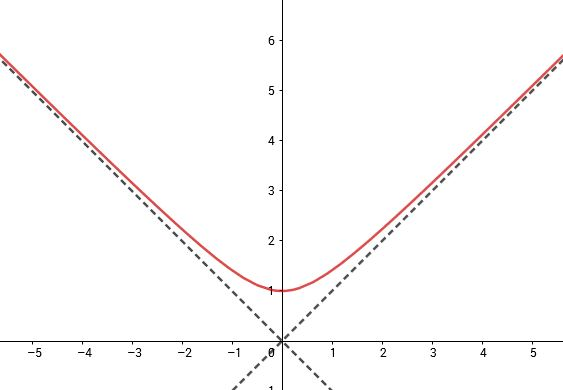
\includegraphics[scale=0.35]{ChapterPowerSeries/Figures/mixedpracticepowerseries1.jpg}
\\ }{0in}
\end{enumerate}
\AnswerKeyEntry{a.)~~$y^2-x^2=1 \rightarrow y^2=\pm\sqrt{1+x^2}$,~~b.)~~$\lim\limits_{x\rightarrow \infty} \frac{f(x)}{x}=1$ and $\lim\limits_{x\rightarrow \infty} \frac{f(x)}{-x}=-1$~~c.)~~$1+1/2 x^2$  a Parabola with vertex at (0,1) and squished by 1/2.}
\end{exercise}

\begin{exercise}{\Coffeecup \Coffeecup \Coffeecup}
\begin{enumerate}[label=\alph*.)]
\item Find a function whose power series is $$1-\frac{1}{2}x^2+\frac{1}{4}x^4-\frac{1}{6}x^6+\frac{1}{8}x^8-\cdots $$
\solushun{Factor out $-\frac{1}{2}$ to get $1-\frac{1}{2} \left( x^2+\frac{1}{2}x^4-\frac{1}{3}x^6+\frac{1}{4}x^8-\cdots\right) = 1-\frac{1}{2} \sum\limits_{n=1}^{\infty} {(-1)^{n+1}\frac{1}{n}x^{2n}}$  Notice $\sum\limits_{n=1}^{\infty} {(-1)^{n+1}\frac{1}{n}x^{2n}}$ looks very similar to $\ln{x} =  \sum\limits_{n=1}^{\infty} {(-1)^{n+1}\frac{1}{n}(x-1)^{n}}$ we just need to reconcile how $(x-1)^n \Longleftrightarrow x^{2n} = (x^2)^n$   Note that $((1+x^2)-1)^n = x^{2n} $ so this is $\ln{(1+x^2)}=\sum\limits_{n=1}^{\infty} {(-1)^{n+1}\frac{1}{n}x^{2n}}$ so we have $1-\frac{1}{2}x^2+\frac{1}{4}x^4-\frac{1}{6}x^6+\frac{1}{8}x^8-\cdots =1-\frac{1}{2} \sum\limits_{n=1}^{\infty} {(-1)^{n+1}\frac{1}{n}x^{2n}} = 1-\frac{1}{2} \ln{(1+x^2)} $
\\ }{0in}

\item Find the Interval of Convergence for the series from part a).  

\solushun{We can use the ratio test to look at the IOC. $\lim\limits_{n \to \infty}{\left|\frac{(-1)^{n+2} x^{2n+2}}{(n+1)} \cdot \frac{n}{(-1)^{n+1} x^{2n}}\right|}=\lim\limits_{n \to \infty}{\frac{n}{n+1} \cdot (x^2)}=x^2$  So we just need to find which values of x will let $x^2<1$ since the ratio test tells us that the series will converge where the limit is less than 1.  This yields an IOC of (-1,1).  WE now need to explore the end points using other tests since at 1 or -1 the ratio test will give no information. \\
The Alternating series test gives us the best solution since when$x=1 or x=-1$ the series is $\sum\limits_{n=1}^{\infty} {(-1)^{n+1}\frac{1}{n}}$ where $a_n = \frac{1}{n}$ which goes to zero as n goes to infinity and so the series converges. which means our final IOC is [-1,1].
\\ }{0in}
\end{enumerate}
\AnswerKeyEntry{a.~~ $1-\frac{1}{2} \ln{(1+x^2)} $ 
b.~~ [-1,1]
}
\end{exercise}


\begin{exercise}{Yet More Practice! \Coffeecup \Coffeecup \Coffeecup}
\begin{itemize}

\item \begin{itemize} \item Find a degree two power series for the function $ \sqrt[3]{x} $ centered at 8. 
 
\vspace*{2in}

\item Use your approximation from part a) to estimate the value of $\sqrt[3]{8.05}$.

\vspace*{2in}

\item Use Taylor's Error Theorem to give a bound on how bad the error could be in your estimation of the value of $\sqrt[3]{8.05}$.  Type the exact value into a calculator or CAS and confirm that you have obtained the desired accuracy.

\vspace*{2in}

\end{itemize}

\item Evaluate each of the following infinite series to a closed form.  Explain your reasoning. \begin{itemize}
\item  $ \overset{\infty}{\underset{n=0}{\sum}} \frac{3^n}{n!2^{n+1}}$

\vspace*{1.5in}

\item $ \overset{\infty}{\underset{n=3}{\sum}} \frac{(-1)^n}{n} $

\vspace*{1.5in}

\item $ \overset{\infty}{\underset{n=0}{\sum}} \frac{(-1)^{n}\pi^{2n}}{(2n)!2^{2n}} $

\vspace*{1.5in}

\end{itemize}
\begin{comment}

\item  \begin{itemize} \item List by hand how many ways you could make change for 35 cents using nickels, dimes, and quarters.

\vspace*{2in}

\item Show how you would use geometric series as generating functions to reach this same conclusion.  Verify your answers match.

\vspace*{3in}
\end{itemize}

\end{comment}
\item Find a rational number that approximates the square root of $e$ accurate to three decimal places.  ({\bf Hint:} Think of the function $e^{x}$ evaluated at $x={1/2}$.  Then use Taylor's Error Theorem to guarantee sufficient accuracy.)
\vspace*{3in}

\item Find power series and Interval of Convergence for the following functions:

\begin{itemize} \item $f(x)=\frac{1}{x}$ centered at -3

\vspace*{1in}

\item $f(x)=\frac{1}{1-x}$ centered at -3

\vspace*{1in}

\item $f(x)=\frac{1}{e^x}$ centered at 0

\vspace*{1in}

\item $f(x)=\frac{1-x-x^2}{1-x}$ centered at 0

\vspace*{1in}

\item $f(x)=2^x$ centered at 1

\vspace*{1in}

\item $f(x)=x^2+x+1 $ centered at 5

\vspace*{1in}

\end{itemize}

\item  Find a degree three power series centered at zero for the function $\frac{1}{4-x^2}$ in five different ways:
 \begin{itemize}
\item Brute force.

\vspace*{2in}

\item Via geometric series with a substitution for $x$.  

\vspace*{2in}

\item Via a multiplication of the series for $\frac{1}{2-x}$ with 
$\frac{1}{2+x}$.

\vspace*{2in}

\item Via a sum of the series that result in a partial fraction decomposition of $\frac{1}{4-x^2}$.

\vspace*{2in}

\item Via long division, dividing the numerator 1 by the denominator $4-x^2$.

\vspace*{2in}

\end{itemize}
\end{itemize}
\end{exercise}
